\documentclass[tikz,border=3mm,multi=tikzpicture]{standalone}
\usepackage[utf8]{inputenc}
\usepackage[T1]{fontenc}
\usepackage{helvet}
\renewcommand{\familydefault}{\sfdefault}
\usepackage{tikz}
\usetikzlibrary{angles,quotes,calc,intersections}
\begin{document}

\tikzset{every node/.append style={font=\sffamily\small}}
% TikZ 1
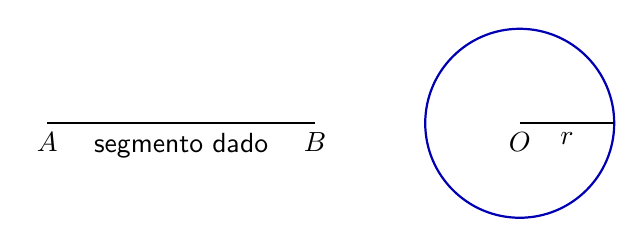
\begin{tikzpicture}[scale=1]
\coordinate (A) at (0,0); \coordinate (B) at (3.4,0);
\draw[thick] (A)--(B);
\node[below] at (A) {$A$}; \node[below] at (B) {$B$};
\node[below] at (1.7,0) {segmento dado};
\coordinate (O) at (6,0);
\draw[thick,blue!70!black] (O) circle (1.2);
\draw[thick] (O)--(7.2,0);
\node[below] at (O) {$O$};
\node[below] at (6.6,0) {$r$};
\end{tikzpicture}
% TikZ 2
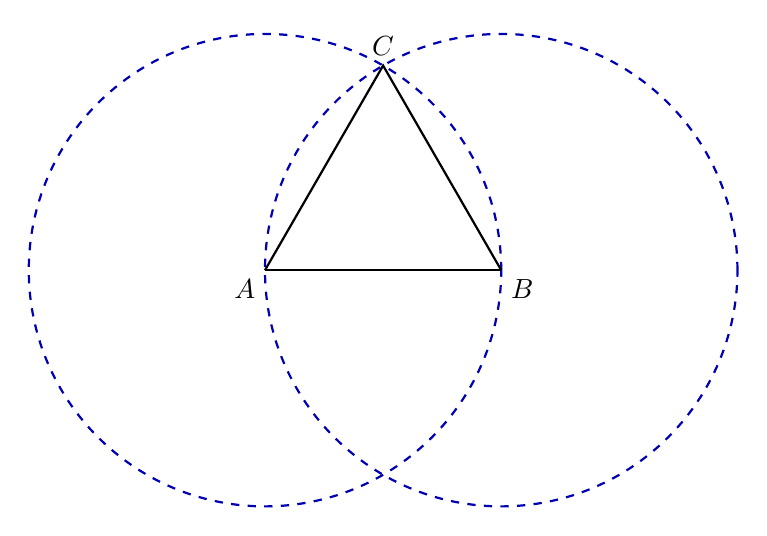
\begin{tikzpicture}[scale=1]
\coordinate (A) at (0,0); \coordinate (B) at (3,0); \coordinate (C) at (1.5,2.598);
\draw[thick] (A)--(B);
\draw[blue!70!black,thick,dashed] (A) circle (3);
\draw[blue!70!black,thick,dashed] (B) circle (3);
\draw[thick] (A)--(C)--(B);
\foreach \p/\pos in {A/below left,B/below right,C/above}{\node[\pos] at (\p) {$\p$};}
\end{tikzpicture}


% TikZ 3
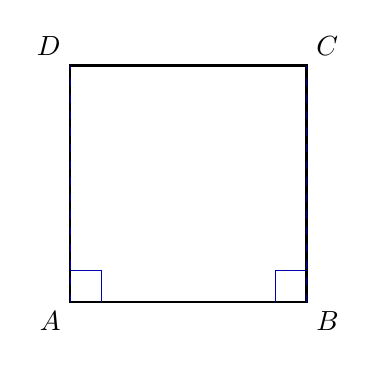
\begin{tikzpicture}[scale=1]
\coordinate (A) at (0,0); \coordinate (B) at (3,0); \coordinate (C) at (3,3); \coordinate (D) at (0,3);
\draw[thick] (A)--(B)--(C)--(D)--cycle;
\draw[blue!70!black,dashed] (A)--(D);
\draw[blue!70!black,dashed] (B)--(C);
\pic[draw=blue!70!black, angle radius=4mm] {right angle=D--A--B};
\pic[draw=blue!70!black, angle radius=4mm] {right angle=A--B--C};
\foreach \p/\pos in {A/below left,B/below right,C/above right,D/above left}{\node[\pos] at (\p) {$\p$};}
\end{tikzpicture}
% TikZ 4
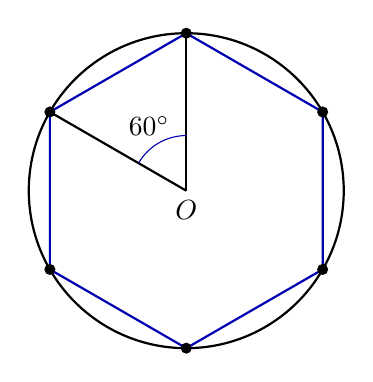
\begin{tikzpicture}[scale=1]
\coordinate (O) at (0,0);
\draw[thick] (O) circle (2);
\foreach \k in {1,...,6}{\coordinate (P\k) at ({90+60*(\k-1)}:2);}
\draw[thick,blue!70!black] (P1)--(P2)--(P3)--(P4)--(P5)--(P6)--cycle;
\foreach \k in {1,...,6}{\fill (P\k) circle (2pt);}
\draw[thick] (O)--(P1);
\draw[thick] (O)--(P2);
\pic[draw=blue!70!black, "$60^{\circ}$", angle radius=7mm, angle eccentricity=1.35] {angle=P1--O--P2};
\node[below] at (O) {$O$};
\end{tikzpicture}


% TikZ 5
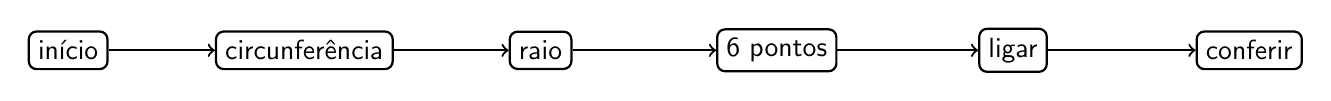
\begin{tikzpicture}[scale=1]
\node[draw,thick,rounded corners=1mm] (I) at (0,0) {início};
\node[draw,thick,rounded corners=1mm] (C) at (3,0) {circunferência};
\node[draw,thick,rounded corners=1mm] (R) at (6,0) {raio};
\node[draw,thick,rounded corners=1mm] (P) at (9,0) {6 pontos};
\node[draw,thick,rounded corners=1mm] (L) at (12,0) {ligar};
\node[draw,thick,rounded corners=1mm] (F) at (15,0) {conferir};
\draw[->,thick] (I)--(C);
\draw[->,thick] (C)--(R);
\draw[->,thick] (R)--(P);
\draw[->,thick] (P)--(L);
\draw[->,thick] (L)--(F);
\end{tikzpicture}
\end{document}
